\section{Ablation Study}
\label{app:ablation}

\begin{center}
\refstepcounter{table}\label{tab:app_per_emotion_asr}
{\footnotesize \MakeUppercase{\tablename}~\thetable}\\
{\scriptsize Per-emotion targeted ASR on the matched-subset pool.  Source
emotion is the ground-truth label of the clean audio; the attack target is
\texttt{happy}.  Pending cells are reserved for the next completed
per-emotion breakdown.}\par
\vspace{2pt}
\centering
\scriptsize
\setlength{\tabcolsep}{3pt}
\resizebox{\columnwidth}{!}{%
\begin{tabular}{l c c c c c}
\toprule
\textbf{Source emotion} & \textbf{Voxtral} & \textbf{OpenS2S} & \textbf{MERaLiON} & \textbf{SALMONN} & \textbf{Kimi-Audio} \\
\midrule
Angry    & 92.20 & 71.21 & \textbf{100.00} & pending & pending \\
Neutral  & 92.00 & 81.10 & \textbf{100.00} & pending & pending \\
Sad      & 96.00 & 81.54 & \textbf{100.00} & pending & pending \\
Surprise & 95.00 & 80.58 & \textbf{100.00} & pending & pending \\
\midrule
\textbf{Overall} & \textbf{93.80} & \textbf{78.44} & \textbf{100.00} & pending & pending \\
\bottomrule
\end{tabular}}
\end{center}

\section{Attack Configuration Details}
\label{app:attack_config}

This appendix lists the settings needed to reproduce the attacks and
evaluations in Section~\ref{sec:experiments}.  When a model-specific
configuration is not available in the local artifacts, we leave the
corresponding entry blank rather than infer it.

\begin{center}
\refstepcounter{table}\label{tab:app_attack_config}
{\footnotesize \MakeUppercase{\tablename}~\thetable}\\
{\scriptsize White-box settings used to generate adversarial audio.  Blank cells
denote settings not found in the available local artifacts.}\par
\vspace{2pt}
\centering
\tiny
\setlength{\tabcolsep}{2.3pt}
\resizebox{\columnwidth}{!}{%
\begin{tabular}{l c c c c c}
\toprule
\textbf{Setting} & \textbf{Voxtral} & \textbf{OpenS2S} & \textbf{MERaLiON} & \textbf{SALMONN} & \textbf{Kimi-Audio} \\
\midrule
Target emotion & happy & happy & happy & happy & happy \\
Emotion labels & 5 labels & 4 labels & 5 labels & 5 labels & 5 labels \\
$L_\infty$ budget $\epsilon$ & 0.008 & 0.008 & 0.008 &  &  \\
Steps & 60 & 60 & 60 &  &  \\
Window A / B & 20 / 40 & 20 / 40 & 20 / 40 &  &  \\
Optimizer & SGD & Adam & SGD &  &  \\
Learning rate & 0.003 & 0.003 & 0.003 &  &  \\
$\lambda_{\mathrm{emo}}$ & 1.0 & 1.0 & 1.0 &  &  \\
$\lambda_{\mathrm{asr}}$ A / B & $10^{-4}$ / $10^{-2}$ & $10^{-4}$ / $10^{-2}$ & $10^{-4}$ / $10^{-2}$ &  &  \\
$\lambda_{\mathrm{perc}}$ A / B & 0 / $10^{-5}$ & 0 / $10^{-5}$ & 0 / $10^{-5}$ &  &  \\
EoT shift / gain & 160 / $[0.8,1.2]$ & 160 / $[0.8,1.2]$ & 160 / $[0.8,1.2]$ &  &  \\
Sample rate & 16 kHz & 16 kHz & 16 kHz &  &  \\
STFT perceptual loss & 256, 512, 1024 & 256, 512, 1024 & 256, 512, 1024 &  &  \\
\bottomrule
\end{tabular}}
\end{center}

\begin{center}
\refstepcounter{table}\label{tab:app_eval_config}
{\footnotesize \MakeUppercase{\tablename}~\thetable}\\
{\scriptsize Evaluation pools and decision rules.}\par
\vspace{2pt}
\centering
\scriptsize
\setlength{\tabcolsep}{4pt}
\begin{tabularx}{\columnwidth}{l X}
\toprule
\textbf{Item} & \textbf{Setting} \\
\midrule
White-box datasets & IEMOCAP, RAVDESS, and ESD.  Source emotions are angry, neutral, sad, and surprise; the target is happy. \\
Matched subset & 60 samples from each evaluated pool, for 240 samples per model. \\
Full-scale ESD & 25 samples per non-happy emotion and per speaker, over 10 speakers when available. \\
Emotion decision & Each audio is queried with three emotion prompts.  A targeted attack succeeds when at least two normalized labels are happy. \\
Decoding & Temperature is 0.0; emotion outputs use at most 16 new tokens, and ASR outputs use at most 256 new tokens. \\
Semantic preservation & Content is preserved when embedding cosine similarity is at least 0.8. \\
Cross-model transfer & Each source model contributes 240 adversarial samples, evaluated with the same three-prompt rule. \\
Black-box surrogate pools & Voxtral EN: 914; Voxtral CN: 962; OpenS2S EN: 944; OpenS2S CN: 774. \\
Black-box targets & Gemini 2.5 Flash, Gemini 2.5 Pro, Qwen3-Omni-Flash, and Qwen-Omni-Turbo are completed.  OpenAI gpt-audio and Grok Voice Agent API are reserved. \\
Black-box metric & For adversarial audio, we report transfer ASR.  For paired clean audio, we report ground-truth emotion accuracy and the rate of predicting the target label. \\
\bottomrule
\end{tabularx}
\end{center}

\begin{center}
\refstepcounter{table}\label{tab:app_prompt_templates}
{\footnotesize \MakeUppercase{\tablename}~\thetable}\\
{\scriptsize Prompt templates used for emotion recognition and ASR probing.}\par
\vspace{2pt}
\centering
\scriptsize
\setlength{\tabcolsep}{4pt}
\begin{tabularx}{\columnwidth}{l X}
\toprule
\textbf{ID} & \textbf{Template} \\
\midrule
P1 & What is the emotion of this audio? Answer with exactly one word from: \emph{labels}. \\
P2 & Classify the emotion. Output exactly one word: \emph{labels separated by slashes}. \\
P3 & Emotion label only (one word): \emph{labels}. \\
ASR & Transcribe the speech exactly. Output only the transcript. \\
Label set & Voxtral and MERaLiON use \texttt{happy}, \texttt{sad}, \texttt{angry}, \texttt{neutral}, and \texttt{surprise}.  OpenS2S uses the same template without \texttt{surprise}. \\
System prompt & OpenS2S uses ``You are a helpful assistant.'' Voxtral and MERaLiON do not define a system prompt in the local configuration. \\
\bottomrule
\end{tabularx}
\end{center}

\begin{center}
\refstepcounter{table}\label{tab:app_blackbox_clean}
{\footnotesize \MakeUppercase{\tablename}~\thetable}\\
{\scriptsize Black-box clean baseline and adversarial transfer metrics.  Values
are percentages.}\par
\vspace{2pt}
\centering
\tiny
\setlength{\tabcolsep}{3pt}
\resizebox{\columnwidth}{!}{%
\begin{tabular}{l l r r r}
\toprule
\textbf{Surrogate} & \textbf{Target} & \textbf{Clean acc.} & \textbf{Clean target rate} & \textbf{Adv. ASR} \\
\midrule
OpenS2S CN & Gemini Flash & 8.91 & 6.20 & 10.72 \\
OpenS2S CN & Gemini Pro & 6.85 & 4.26 & 0.00 \\
OpenS2S CN & Qwen3 & 5.56 & 7.49 & 32.30 \\
OpenS2S CN & Qwen Turbo & 4.91 & 7.62 & 37.34 \\
OpenS2S EN & Gemini Flash & 4.77 & 2.12 & 5.93 \\
OpenS2S EN & Gemini Pro & 4.13 & 2.65 & 0.00 \\
OpenS2S EN & Qwen3 & 29.98 & 8.37 & 14.09 \\
OpenS2S EN & Qwen Turbo & 34.11 & 7.94 & 22.78 \\
Voxtral CN & Gemini Flash & 0.00 & 0.00 & 9.36 \\
Voxtral CN & Gemini Pro & 0.00 & 0.10 & 0.94 \\
Voxtral CN & Qwen3 & 24.01 & 25.57 & 30.98 \\
Voxtral CN & Qwen Turbo & 46.88 & 18.19 & 34.20 \\
Voxtral EN & Gemini Flash & 4.27 & 0.98 & 7.88 \\
Voxtral EN & Gemini Pro & 0.00 & 0.00 & 12.47 \\
Voxtral EN & Qwen3 & 29.32 & 8.86 & 19.69 \\
Voxtral EN & Qwen Turbo & 33.26 & 8.64 & 33.15 \\
\bottomrule
\end{tabular}}
\end{center}

\begin{center}
\refstepcounter{table}\label{tab:app_blackbox_emotion}
{\footnotesize \MakeUppercase{\tablename}~\thetable}\\
{\scriptsize Per-emotion black-box transfer ASR by surrogate and target.  Values
are percentages.}\par
\vspace{2pt}
\centering
\tiny
\setlength{\tabcolsep}{2.5pt}
\resizebox{\columnwidth}{!}{%
\begin{tabular}{l l r r r r}
\toprule
\textbf{Surrogate} & \textbf{Target} & \textbf{Angry} & \textbf{Sad} & \textbf{Neutral} & \textbf{Surprise} \\
\midrule
OpenS2S CN & Gemini Flash & 11.86 & 8.63 & 5.08 & 17.24 \\
OpenS2S CN & Gemini Pro & 0.00 & 0.00 & 0.00 & 0.00 \\
OpenS2S CN & Qwen3 & 30.51 & 32.99 & 23.35 & 41.87 \\
OpenS2S CN & Qwen Turbo & 29.38 & 31.98 & 28.43 & 58.13 \\
OpenS2S EN & Gemini Flash & 7.52 & 3.72 & 2.09 & 10.55 \\
OpenS2S EN & Gemini Pro & 0.00 & 0.00 & 0.00 & 0.00 \\
OpenS2S EN & Qwen3 & 16.37 & 14.46 & 12.13 & 13.50 \\
OpenS2S EN & Qwen Turbo & 23.89 & 17.77 & 17.57 & 32.07 \\
Voxtral CN & Gemini Flash & 10.97 & 6.61 & 5.44 & 14.34 \\
Voxtral CN & Gemini Pro & 3.80 & 0.00 & 0.00 & 0.00 \\
Voxtral CN & Qwen3 & 26.58 & 30.58 & 25.52 & 40.98 \\
Voxtral CN & Qwen Turbo & 32.91 & 22.73 & 25.94 & 54.92 \\
Voxtral EN & Gemini Flash & 8.48 & 5.04 & 5.88 & 12.12 \\
Voxtral EN & Gemini Pro & 37.95 & 0.00 & 13.12 & 0.00 \\
Voxtral EN & Qwen3 & 22.32 & 20.59 & 15.84 & 19.91 \\
Voxtral EN & Qwen Turbo & 35.71 & 30.67 & 27.15 & 38.96 \\
\bottomrule
\end{tabular}}
\end{center}

Figure~\ref{fig:app_convergence_steps} shows the cumulative share of samples
that have converged by each optimization step.  We include local runs that
record this metadata.  Voxtral converges quickly on the ESD EN/CN pools
(1998/2000 converged, mean 5.4 steps).  OpenS2S converges later and less often
on the ESD-final pool (4282/8949 converged, mean 39.5 steps).

\begin{center}
\refstepcounter{figure}\label{fig:app_convergence_steps}
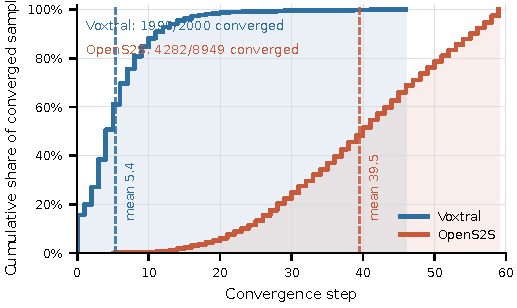
\includegraphics[width=0.98\columnwidth]{figure/appendix_convergence_steps.pdf}
{\scriptsize \textbf{\figurename~\thefigure.} Cumulative convergence profile for
Voxtral and OpenS2S white-box attacks.}\par
\end{center}

\section{Dataset \& Preprocessing Details}
\label{app:dataset_preprocessing}

We construct a small Gemini TTS dataset to study semantic--prosodic emotion
conflict under controlled audio conditions.  For each text prompt, the lexical
content stays fixed across variants.  Only the TTS style instruction changes
the intended prosody.  This gives paired utterances where the semantic emotion
and the prosodic emotion can either agree or conflict, which helps analyze how
audio-language models resolve affective cues.

\begin{center}
\refstepcounter{table}\label{tab:app_tts_dataset}
{\footnotesize \MakeUppercase{\tablename}~\thetable}\\
{\scriptsize Gemini TTS dataset construction and preprocessing summary.}\par
\vspace{2pt}
\centering
\scriptsize
\setlength{\tabcolsep}{4pt}
\begin{tabularx}{\columnwidth}{l X}
\toprule
\textbf{Item} & \textbf{Description} \\
\midrule
Generation source & Gemini TTS.  The exact voice and model identifiers are not fixed in the available artifacts. \\
Languages & English and Chinese prompts. \\
Semantic prompts & About 50 short prompts.  The lexical content is kept fixed across prosodic variants. \\
Prosody labels & Five intended styles: \texttt{neutral}, \texttt{happy}, \texttt{sad}, \texttt{angry}, and \texttt{surprise}. \\
Candidate size & Approximately 250 candidate utterances, obtained by rendering each prompt under the five prosodic styles. \\
Conflict construction & Consistent pairs use matching semantic and prosodic labels.  Conflict pairs use different semantic and prosodic labels. \\
Filtering & We exclude failed synthesis, incomplete audio, and samples with unusable speech quality. \\
Preprocessing & Audio is converted to the waveform format required by the evaluation pipeline.  Labels are normalized to the five-emotion vocabulary above. \\
\bottomrule
\end{tabularx}
\end{center}

\begin{samepage}
\section{Additional Attack Examples}
\label{app:additional_examples}

Table~\ref{tab:app_attack_examples} gives representative examples recovered
from the white-box per-sample JSON files.  It is not an aggregate result.
Instead, it shows how the majority emotion vote and ASR text change for
individual clean--adversarial pairs.  The selected rows cover preserved
successes, semantic-damage successes, and boundary cases.

\begin{center}
\refstepcounter{table}\label{tab:app_attack_examples}
{\footnotesize \MakeUppercase{\tablename}~\thetable}\\
{\scriptsize Representative clean--adversarial examples.  Vote entries use
A=angry, N=neutral, S=sad, and H=happy.}\par
\vspace{2pt}
\centering
\tiny
\setlength{\tabcolsep}{2pt}
\begin{tabularx}{\columnwidth}{l l l c c X X c}
\toprule
\textbf{Case} & \textbf{Pool} & \textbf{Src.$\rightarrow$Tgt.} & \textbf{Clean} & \textbf{Adv.} & \textbf{Clean ASR} & \textbf{Adv. ASR} & \textbf{Sim./SNR} \\
\midrule
Stealth & Voxtral/ESD-EN & angry$\rightarrow$happy & N/H/H & H/H/H & Over them swoop the Eagles. & Over them swoop the Eagles. & 1.00/31.6 \\
Damage & Voxtral/IEMOCAP & angry$\rightarrow$happy & A/A/A & H/H/H & I am sick and tired of listening to you \ldots & I am pickin' tides of listenin' to you \ldots & 0.56/28.7 \\
Near miss & Voxtral/IEMOCAP & angry$\rightarrow$happy & N/N/N & N/H/H & Then it isn't just my business. & And then it isn't just my business. & 1.00/17.2 \\
Stealth & OpenS2S/RAVDESS & angry$\rightarrow$happy & A/A/A & H/H/H & Dogs are sitting by the door. & Dogs are sitting by the door. & 1.00/25.2 \\
Damage & OpenS2S/IEMOCAP & angry$\rightarrow$happy & A/A/A & H/H/H & Nobody comes 700 miles \ldots & The car traveled 700 miles. & 0.37/4.9 \\
Near miss & OpenS2S/RAVDESS & angry$\rightarrow$happy & A/A/A & N/N/N & Dogs are sitting by the door. & Dogs are sitting by the door. & 1.00/15.9 \\
\bottomrule
\end{tabularx}
\end{center}

Figure~\ref{fig:app_waveform_spectrogram} shows one recovered Voxtral ESD pair.
The visualization is generated from the local clean waveform and its recovered
adversarial waveform.  The waveform view shows small global changes, while the
STFT view makes the perturbation easier to inspect.

\begin{center}
\refstepcounter{figure}\label{fig:app_waveform_spectrogram}
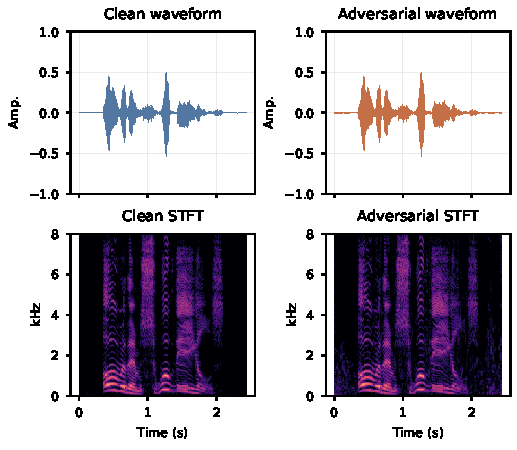
\includegraphics[width=0.86\columnwidth]{figure/appendix_waveform_spectrogram.pdf}
{\scriptsize \textbf{\figurename~\thefigure.} Clean versus adversarial waveform
and STFT comparison for a recovered Voxtral ESD sample.}\par
\end{center}
\end{samepage}
